\part{Numerical Exercises}

\chapter{Getting started with MOLE}

The official website is \url{https://csrc-sdsu.github.io/mole}.
After skimming the description and reading the papers you will find out that this method never uses a ghost points.

\section{Compiling and running the first code}
% https://www.csrc.sdsu.edu/research-reports

\subsection{Create the staggered grid}

\section{Transport 1D}

\begin{equation*}
    \diffp{u}{t}+c\diffp{u}{x}=
    0.
\end{equation*}

\begin{listing}[ht!]
    \tiny
    \centering
    \pathinputminted[frame=single,framesep=10pt,linenos,firstline=9,lastline=35,highlightlines={9}]{cpp}{hyperbolic1D_upwind.cpp}
    \caption{Programa~\texttt{hyperbolic1Dupwind.cpp}}
    \label{code:hyperbolic1Dupwind.cpp}
\end{listing}

\section{Poisson 1D}

\begin{listing}[ht!]
    \tiny
    \centering
    \pathinputminted[frame=single,framesep=10pt,linenos,firstline=1,lastline=53,highlightlines={21,29}]{octave}{elliptic1D.m}
    \caption{Programa~\texttt{elliptic1D.m}}
    \label{code:elliptic1D.m}
\end{listing}

\begin{equation}\label{eq:poisson1drobindconditions}
    \left\{
    \begin{aligned}
        \diff[2]{u}{x}
         & =e^{x},
        \text{ para }x\in\left[0,1\right].     \\
        0
         & = u\left(0\right)-\diff{u}{x}[x=0]. \\
        2e
         & =u\left(1\right)+\diff{u}{x}[x=1].
    \end{aligned}
    \right.
\end{equation}

\begin{itemize}
    \item

          En la línea $1$ encontramos el
          \emph{shebang}\footnote{\url{https://en.wikipedia.org/wiki/Shebang_(Unix)}},
          esto permite ejecutar un script de Octave
          \mintinline{bash}|./elliptic1D.m| con la opción de modo de
          procesamiento por lotes (batch), para esto se necesita
          tener permisos de ejecución (por ejemplo,
          \mintinline{bash}|chmod +x elliptic1D.m|).

    \item

          En las líneas $2$ al $10$ tenemos un comentario sobre el
          programa de modo que ayude al codificador a obtener un
          contexto del problema a resolver.

    \item

          En la línea $12$, la función
          \href{https://docs.octave.org/v9.3.0/Manipulating-the-Load-Path.html#index-addpath}{\mintinline{octave}|addpath|}
          agrega el directorio
          \mintinline{octave}|"/usr/share/mole/matlab/"| a la ruta de
          búsqueda de la función.
          Allí se encuentran el conjunto de scripts Octave / MATLAB
          de la biblioteca MOLE.
          Vea el Programa~\ref{code:moledirectoriesoctave.txt}.

    \item

          En las líneas $14$ y $15$, se inicializan los identicadores
          \mintinline{octave}|west| (oeste, izquierda),
          \mintinline{octave}|east| (este, derecha) con los valores
          de $0$ y $1$, respectivamente, estos representan los
          valores de frontera del dominio espacial
          en~\eqref{eq:poisson1drobindconditions}.

    \item

          En la línea $21$, llamamos a la función
          \href{https://carlosal1015.github.io/mole_examples/api_docs/matlab/src/matlab/lap.html}{\mintinline{octave}|lap|},
          este genera un operador Laplaciano discreto extendido que
          requiere como argumentos obligatorios el orden de precisión
          \mintinline{octave}|k|, el número  de celdas
          \mintinline{octave}|m| y el tamaño de paso
          \mintinline{octave}|dx|.
          \begin{equation*}
              L=L^{\left(k\right)}=
              D^{\left(k\right)}
              G^{\left(k\right)}=
              DG.\qquad\qquad
              \left(
              \difc.L.{}{}=\nabla\cdot\nabla
              \right),
          \end{equation*}
          donde $D$ y $G$ son los operadores miméticos de divergencia
          y gradiente, respectivamente.
          Dado que
          \begin{math}
              D\in
              \mathbb{R}^{\left(m+2\right)\times\left(m+1\right)}
          \end{math}
          y
          \begin{math}
              G\in
              \mathbb{R}^{\left(m+1\right)\times\left(m+2\right)}
          \end{math},
          entonces
          \begin{math}
              L\in
              \mathbb{R}^{\left(m+2\right)\times\left(m+2\right)}
          \end{math}.

    \item

          En la línea $22$, con la función
          \href{https://docs.octave.org/v9.3.0/Figure-Properties.html#index-figure-visible}{\mintinline{octave}|figure|}
          desactivamos que se muestre la figura en la pantalla,
          preferimos solamente guardar la gráfica.

    \item

          En la línea $23$, con la función
          \href{https://docs.octave.org/latest/Information.html#index-spy}{\mintinline{octave}|spy|}
          graficamos (no se mostrará) el patrón de dispersidad de
          $L$.

          \begin{figure}[ht!]
              \centering
              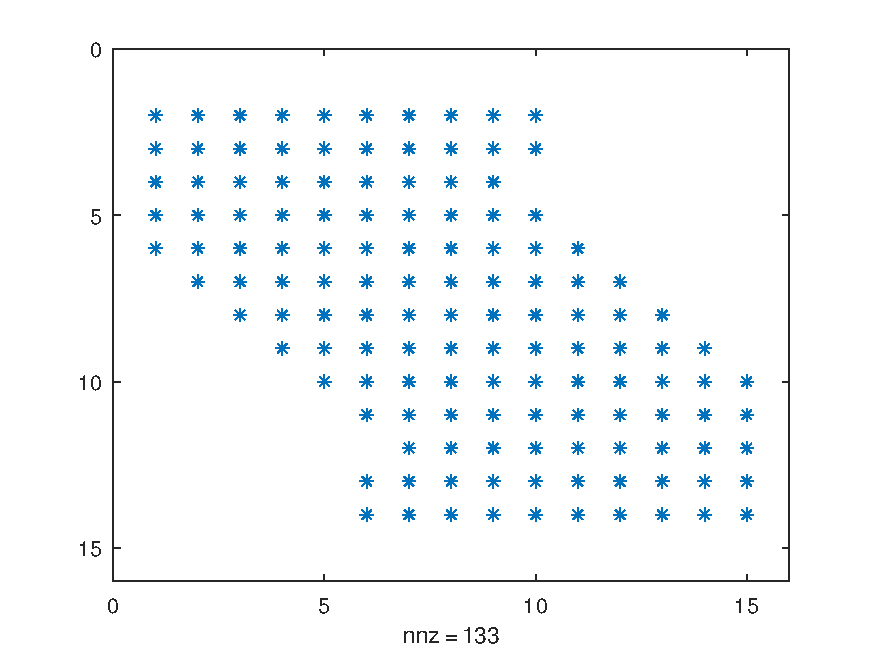
\includegraphics[width=.39\paperwidth]{../examples/octave/elliptic1Dsparsebefore.pdf}
              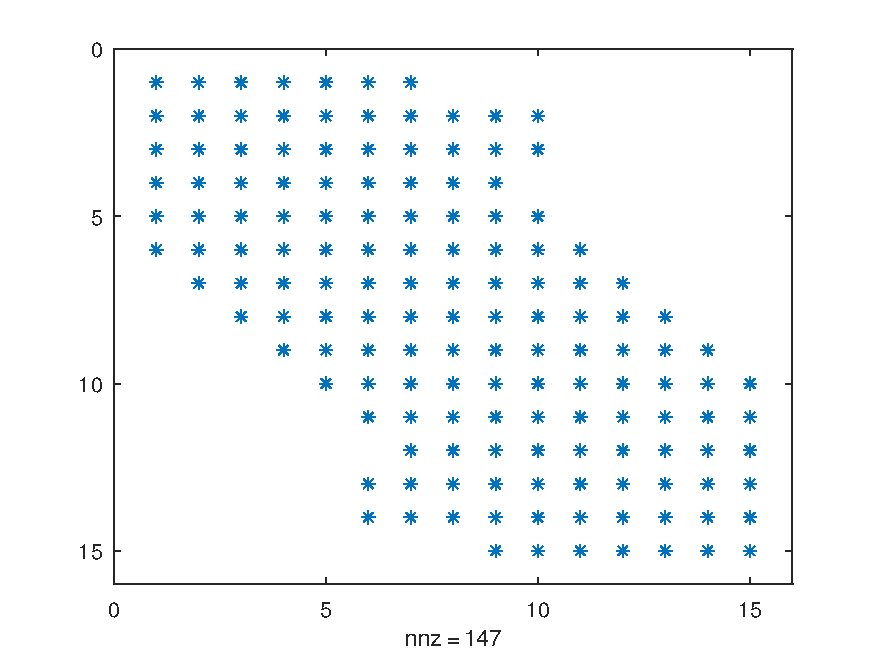
\includegraphics[width=.39\paperwidth]{../examples/octave/elliptic1Dsparseafter.pdf}
              \caption{Izquierda: Representación dispersa de $L$ hasta la línea
                  21.
                  La primera y la última fila son vectores de ceros.
                  Derecha: Representación dispersa de $L$ hasta la línea 29.
                  La matriz $L\in\mathbb{R}^{15\times 15}$.}
          \end{figure}

    \item

          En la línea $24$, con la función
          \href{https://docs.octave.org/latest/Printing-and-Saving-Plots.html}{\mintinline{octave}|saveas|}
          guardamos esta gráfica en formato PDF y recortado.

    \item

          En la línea $29$, llamamos a la función
          \href{https://carlosal1015.github.io/mole_examples/api_docs/matlab/src/matlab/robinBC.html}{\mintinline{octave}|robinBC|},
          este requiere como argumentos obligatorios el orden de
          precisión \mintinline{octave}|k|, el número  de celdas
          \mintinline{octave}|m|, el tamaño de paso
          \mintinline{octave}|dx|, el coeficiente Dirichlet
          \mintinline{octave}|a| y el coeficiente Neumann
          \mintinline{octave}|b|.
          Esta función devuelve una matriz en
          \begin{math}
              \mathbb{R}^{\left(m+2\right)\times\left(m+2\right)}
          \end{math}.
          Actualizamos la matriz \mintinline{octave}|L| según el
          Algoritmo~\ref{algo:updateL}.

          \begin{algorithm}[H]
              \caption{Actualizaciones del operador Laplaciano discreto extendido.}\label{algo:updateL}
              $A\leftarrow L$\;
              $F\leftarrow f$\;
              $A\leftarrow A+R_{G}$\;
              $U\leftarrow \text{solve}\left(A, F\right)$\;
          \end{algorithm}

    \item

          En la línea $34$, creamos la malla escalonada
          unidimensional, note que los puntos internos son los
          centros de las celdas equiespaciados por
          \mintinline{octave}|dx|.
          La distancia entre el extremo izquierdo y el posterior
          punto malla, así como del extremo derecho y el anterior
          punto malla es \mintinline{octave}|dx/2|.

    \item

          En las líneas $35$ y $43$, guardamos
          \href{https://docs.octave.org/latest/Simple-File-I_002fO.html#index-save-6}{\mintinline{octave}|save|}
          la malla computacional y la solución en el formato HDF5
          para posterior post procesamiento.

    \item

          En la líneas $39$ y $40$, aplicamos las condiciones de
          frontera Robin, empleamos la función
          \href{https://docs.octave.org/latest/Exponents-and-Logarithms.html#XREFexp}{\mintinline{octave}|exp|}.
          El signo menos que antecede al coeficiente Neumann
          \mintinline{octave}|b| se debe a que en el borde izquierdo
          de la malla el vector normal hacia afuera apunta hacia la
          izquierda, mientras que en el borde derecho el vector
          normal hacia afuera apunta hacia la derecha.

    \item

          En la línea $42$, resolvemos el sistema de ecuaciones lineales
          disperso con la función \href{https://docs.octave.org/latest/Arithmetic-Ops.html#index-mldivide}{\mintinline{octave}|mldivide|}.

          \begin{figure}[ht!]
              \centering
              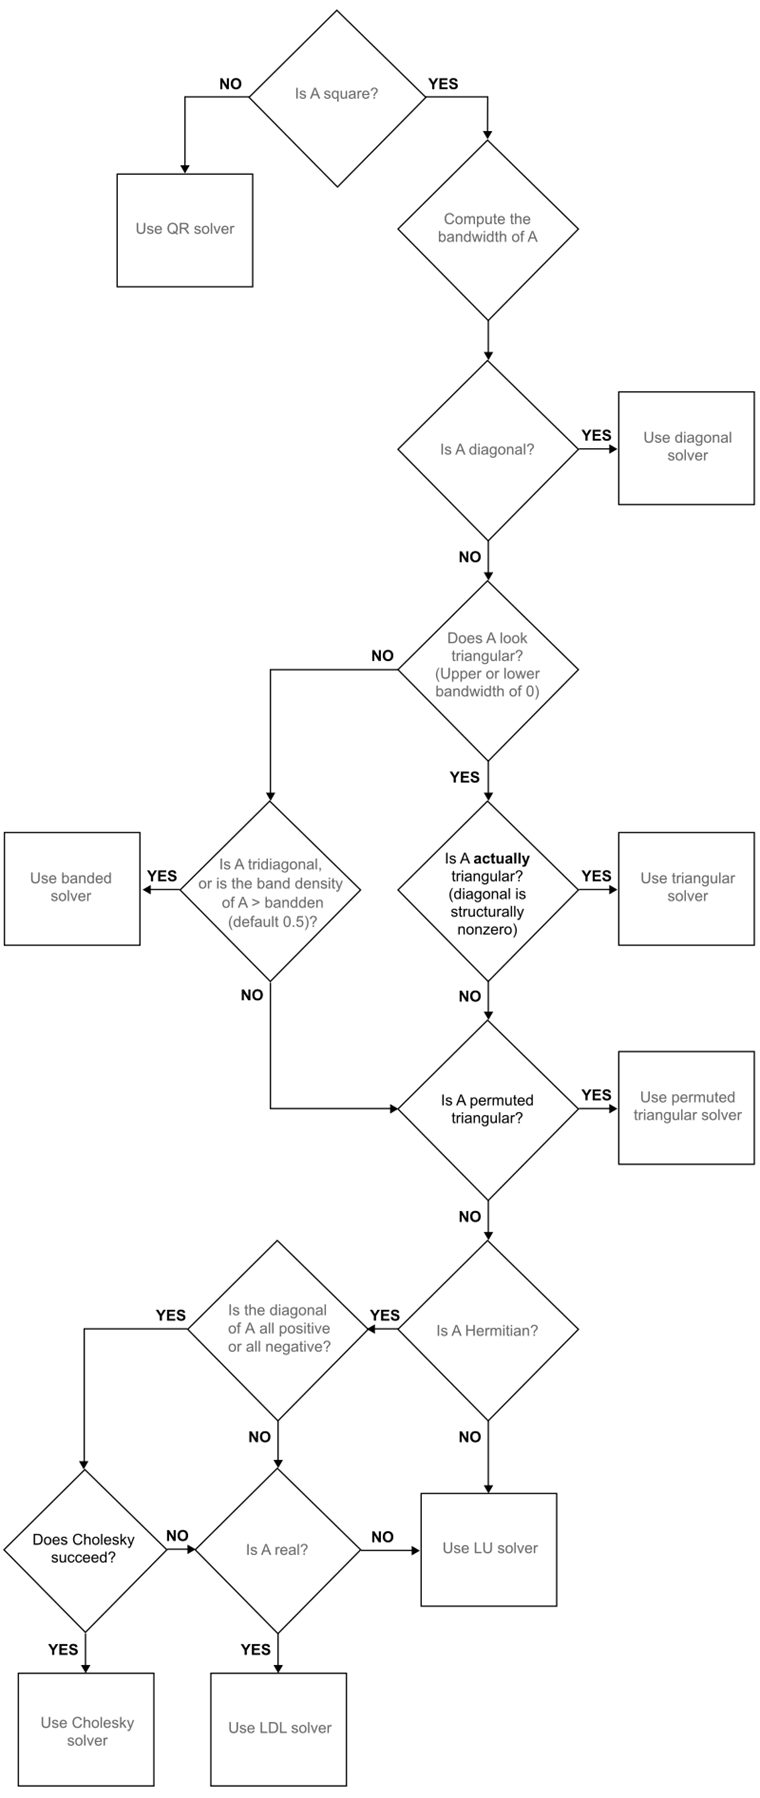
\includegraphics[width=.3\paperwidth]{mldivide_sparse}
              \caption{Diagrama de flujo del solucionador
                  \mintinline{octave}|mldivide| para matrices
                  disperas que emplea MATLAB.
                  Recuperado de~\url{https://www.mathworks.com/help/matlab/ref/double.mldivide.html}.}
          \end{figure}
\end{itemize}

\section*{Resultados del Programa~\ref{code:elliptic1D.m}}

En primer lugar, mostramos la gráfica a escala 1:1 de la solución
exacta y de la solución mimética obtenida en el Programa~\ref{code:elliptic1D.m}.

\begin{figure}[ht!]
    \centering
    % \includegraphics[width=.6\paperwidth]{../examples/octave/elliptic1D.pdf}
    \includegraphics[width=.39\paperwidth]{elliptic1D.pdf}
    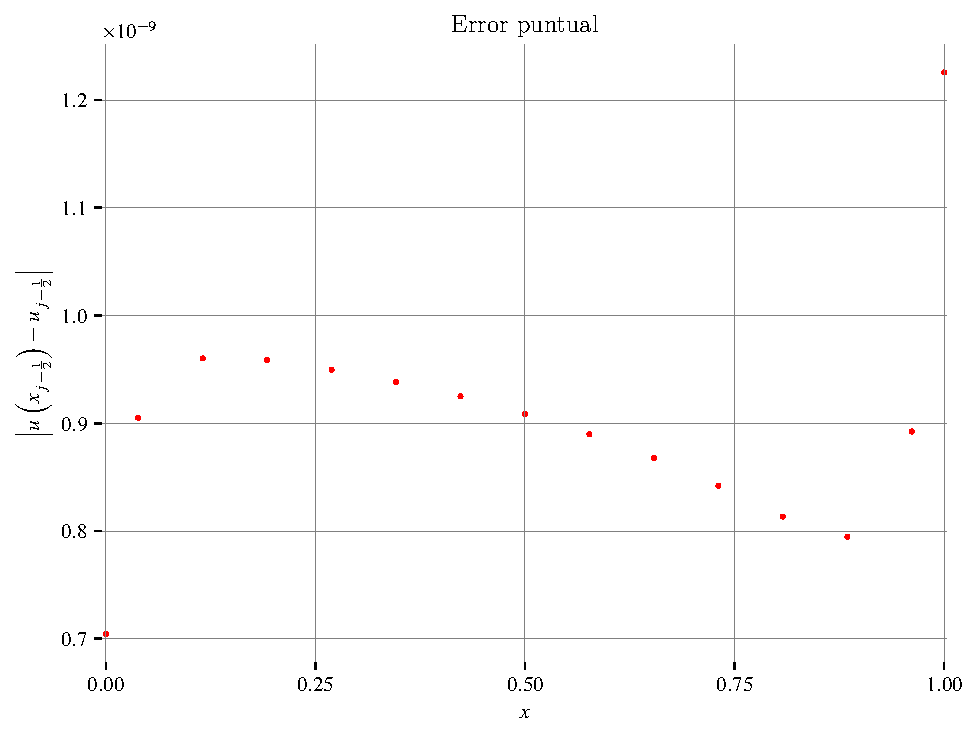
\includegraphics[width=.39\paperwidth]{elliptic1Derror.pdf}
    \caption{Izquierda: Solución de~\eqref{eq:poisson1drobindconditions}
        usando \mintinline{octave}|k=6| y \mintinline{octave}|m=2k+1=13|.
        Derecha: Error en la malla escalonada
        \begin{math}
            \left\{
            0,
            \dotsc,
            x_{j-\frac{1}{2}}
            \dotsc,
            1
            \right\}
        \end{math}}
\end{figure}

En segundo lugar, mostramos una gráfica del error en cada punto de la malla computacional
dada por
\begin{equation*}
    \text{Error de $u$ en $x_{j-\frac{1}{2}}$}=
    \left|
    u\left(x_{j-\frac{1}{2}}\right)-
    u_{j-\frac{1}{2}}
    \right|.
\end{equation*}

Por último, mostramos la tabla de los errores y el orden de convergencia numérico.

\begin{table}[ht!]
    \centering
    \begin{tabular}{ccc}
        \toprule
        $\Delta x$            & Error $\ell_1$        & Orden    \\
        \midrule
        $1.562\times 10^{-2}$ & $4.410\times 10^{-2}$ & -        \\
        $1.535\times 10^{-2}$ & $4.464\times 10^{-2}$ & $-0.678$ \\
        \bottomrule
    \end{tabular}
    \caption{Tabla de errores de aproximación de $U$ en
        $x_{j-\frac{1}{2}}$ y el orden convergencia numérico obtenido.}
    \label{table:errors}
\end{table}


\section{The 1D Diffusion Equation}

Given the one-dimensional heat equation

\begin{equation}\label{eq:IBVPheat1d}
    \begin{cases}
        \diffp{u}{t}=
        \kappa\diffp[2]{u}{x},
                                      & \left(x,t\right)\in
        \left(a,b \right)\times\left(0, \infty \right).     \\
        u\left(x,0\right)=f(x),
                                      & x\in
        \left[a,b\right].                                   \\
        u\left(a,t\right)= \alpha(t), & t\in
        \left(0,\infty\right),                              \\
        u\left(b,t\right)= \beta(t),
                                      & t\in
        \left(0,\infty\right),
    \end{cases}
\end{equation}

where $\kappa$ is the thermal diffusivity.\\

The 1D heat equation code by mimetic methods


\begin{listing}[ht!]
    \tiny
    \centering
    \pathinputminted[frame=single,framesep=12pt,linenos,firstline=1,lastline=80,highlightlines={20,29}]{octave}{parabolic1D.m}
    \caption{Programa~\texttt{parabolic1D.m}}
    \label{code:parabolic1D.m}
\end{listing}


In the one-dimensional heat equation in the parabolic1D.m code, the PDE being solved is given by:


\begin{equation}\label{eq:IBVPheat1d}
    \begin{cases}
        \diffp{u}{t}=
        \kappa\diffp[2]{u}{x},
                                 & \left(x,t\right)\in
        \left(0,1 \right)\times\left(0, 1 \right).     \\
        u\left(x,0\right)= 0,
                                 & x\in
        \left[0,1\right].                              \\
        u\left(0,t\right)= 100., & t\in
        \left(0,1 \right),                             \\
        u\left(1,t\right)= 100.,
                                 & t\in
        \left(0, 1\right),
    \end{cases}
\end{equation}


\textbf{Line 9:} In this part the code defines the value of the diffusion coefficient $\kappa =1$.\\

\textbf{Line 10:} Define the left side $a= 0$ of the domain of the variable $x$.\\

\textbf{Line 11:} Define the right hand side $b= 1$ of the domain of the variable $x$.\\

\textbf{Line 13:} The Operator's order of accuracy $k = 2$.\\

\textbf{Line 14:} $m$ is the number of cells, where $m$ can take values ​​$m \geq 2*k+1$; in this case $m=2*(2)+1=5$.\\

\textbf{Line 15:} In this line the step size in $x$ is defined, defined as $dx=(b-a)/m$, en this case, replacing it, we have $dx =\frac{1-0}{5} =\frac{1}{5}$ \\

\textbf{Line 17:} End time $t=1$.\\

\textbf{Line 18:} Von Neumann stability criterion for $k=2$, we have $ dt = \frac{(dx)^{2}}{3 \kappa}$, in this exercise the step in time is given by: $dt =\frac{1}{75}$\\

\textbf{Line 20:} $L = lap(k,m,dx)$ 1D mimetic Laplacian operator is of order $m+2$ so $m+2$ for this exercise is of order 7 by 7, where $k=2$, $m = 5$ and $\frac{1}{5}$, then $L = lap(2,5,\frac{1}{5})$.\\

\textbf{Line 23:} The initial condition  value $u(x,0)=0$ is a matrix of order $m+2$ by $1$, in this case $7$ by $1$.\\

\textbf{Line 25:} The boundary condition is on the left side u(a,t)= u(0,t)=100\\

\textbf{Line 26:} The boundary condition on the right side u(b,t)= u(1,t)=100\\

\textbf{Line 29:} The mesh used in the mimetic method  grid = $[west$  $west+dx/2: dx :east-dx/2$  $east]$, then grid = $[a$ $a+\frac{dx}{2}: dx : b-\frac{dx}{2}$ $b  ]$, in this exercise the mesh is given by:

\begin{center}

    grid = $[0$ $\frac{1}{10}: \frac{1}{5}: \frac{9}{10}$ $1]$ = $  \{0, \frac{1}{10}, \frac{3}{10}, \frac{5}{10}, \frac{7}{10}, \frac{9}{10}, 1 \}$

\end{center}

\textbf{Line 31:} If explicit=1 then the PDE will be solved in time by the explicit method, and if explicit=0 then the PDE will be solved by the implicit method.\\

\textbf{Line 33 to 50:} In this section we have the explicita solution of the PDE and the graph. \\

\textbf{Line 36:} The value of L is obtained by:

\begin{equation}
    \frac{\partial u}{\partial t} = \kappa \frac{\partial^{2} u}{\partial x^{2}}
\end{equation}

Discretizing $\frac{\partial u}{\partial t}$ by forward finite differences, and $\frac{\partial^{2} u}{\partial x^{2}}$ by applying mimetic methods

\begin{equation}
    \frac{u^{n+1}_{i} - u^{n}_{i} }{dt} = \kappa L 	u^{n}_{i}
\end{equation}

then clearing $u^{n+1}_{i}$ we obtain:


\begin{equation}
    u^{n+1}_{i} = u^{n}_{i}  +  \kappa dt L u^{n}_{i}
\end{equation}

Factoring $u^{n}_{i}$ we have:

\begin{equation}
    u^{n+1}_{i} = (I  +  \kappa dt L )u^{n}_{i}
\end{equation}

where $I$ is the identity matrix of general order $m+2$ by $m+2$, for this exercise of order $7$ by $7$, being

$$  L = (\kappa dt L +I )$$

being in the code: $ L = alpha*dt*L + speye(size(L))$; finally to obtain the solution

\begin{equation}
    u^{n+1}_{i} = L *u^{n}_{i}
\end{equation}

in the code on line 47 we have $ U = L*U.$\\


\textbf{Line 39:} The iteration starts for $t=0$ until $t=t/dt+1$, in this exercise $t/dt+1= 75+1=76$.\\


\textbf{Line 40 and 60:} The graph of the mesh on the $x$ axis by grid and the solution of the PDE $U$. \\


\textbf{Line 41 and 62:} In this line the graph is on the $x$ axis from 0 to 1 and on the $y$ axis from 0 to 105.\\


\textbf{Line 42 and 63:} In this line prints the different times ($ i* dt$)for explicit method, with two decimal  ($ .2f $).\\


\textbf{Line 43 and 64:} Use the title command to display the title designated on line 42. \\


\textbf{Line 44 and 65:} Label the $x$-axis in this exercise as $x$.


\textbf{Line 45 and 66:} Label the $y$-axis in this exercise as $T$.\\


\textbf{Line 46 and 67:} Shows the graph for the different times with a pause of 0.01. \\


\textbf{Line 50 to 71:} In this section we have the implicita solution of the PDE and the graph. \\

\textbf{Line 53:} The value of L is obtained by:

\begin{equation}
    \frac{\partial u}{\partial t} = \kappa \frac{\partial^{2} u}{\partial x^{2}}
\end{equation}

Discretizing $\frac{\partial u}{\partial t}$ by forward finite differences, and $\frac{\partial^{2} u}{\partial x^{2}}$ by applying mimetic methods

\begin{equation}
    \frac{u^{n+1}_{i} - u^{n}_{i} }{dt} = \kappa L 	u^{n+1}_{i}
\end{equation}

then clearing $u^{n+1}_{i}$ we obtain:


\begin{equation}
    u^{n+1}_{i}(I - \kappa dt L ) = u^{n}_{i}
\end{equation}

where $I$ is the identity matrix of general order $m+2$ by $m+2$, for this exercise of order $7$ by $7$, being

$$  L = (-\kappa dt L + I)$$

being in the code: $ L = -alpha*dt*L +speye(size(L))$.\\

\textbf{Line 54:} In this line $dL=$ decomputation($L$) the matrix L is decomposed into lower triangular matrix $L$ and upper triangular matrix $U$ using LU decomposition method.\\

\textbf{Line 68:} In this line solve the $u^{n+1} =(dL)^{-1}*u^{n}$, thus finding the solution $U=dL \setminus U$.\\



\section{Convection-diffusion}
Given the three-dimensional convection diffusion equation

\begin{equation}\label{eq:IBVP3d}
    \begin{cases}
        \diffp{u}{t} + \nabla \cdot (\textbf{v} u) = \nabla \cdot (D \nabla u) + R,
                                      & \textbf{x} \in \Omega, t > 0     \\
        u\left( \textbf{x},0\right)= \bar{\alpha},
                                      & \textbf{x} \in  \Omega.\\
        u\left(\textbf{x},t\right)= \bar{\alpha}_{0}, & t >0, \textbf{x} \in \partial  \Omega  
    \end{cases}
\end{equation}

where  $\Omega$  is the three-dimensional domain with  boundary $\partial  \Omega $.

\begin{listing}[ht!]
    \tiny
    \centering
    \pathinputminted[frame=single,framesep=12pt,linenos,firstline=1,lastline=32,highlightlines={20,29}]{octave}{convection_diffusion.m}
    \caption{Programa~\texttt{convection\_diffusion.m}}
    \label{code:convection_diffusion.m}
\end{listing}

\textbf{Line 11:} The Operator's order of accuracy $k = 2$.\\

\textbf{Line 12:} $m$ is the number of cells on the x-axis, where $m$ can take values ​​$m= 101$.\\

\textbf{Line 13:} $m$ is the number of cells on the y-axis, where $m$ can take values ​​$m= 51$.\\

\textbf{Line 14:} $m$ is the number of cells on the z-axis, where $m$ can take values ​​$m= 101$.\\

\textbf{Line 17 and 18:} The domain on the  x-axis, $a=0 \leq x \leq 101=b$\\

\textbf{Line 19 and 20:} The domain on the  y-axis, $c=0 \leq y \leq 51=d$\\

\textbf{Line 21 and 22:} The domain on the  z-axis, $e=0 \leq x \leq 101=f$\\

\textbf{Line 25:} The spatial step sizes on the x-axis, $ dx = (b-a)/m$, this case $dx = 1$.\\

\textbf{Line 26:} The spatial step sizes on the y-axis, $ dy = (d-c)/n$, this case $dy = 1$.\\

\textbf{Line 27:} The spatial step sizes on the z-axis, $ dz = (f-e)/o$, this case $dz = 1$.\\

\textbf{Line 30:} three-dimensional mimetic divergence operator $div3D(k,m,dx,n,dy,o,dz)=div3D(2,101,1,51,1,101,1)$\\

\textbf{Line 31:} three-dimensional mimetic gradient operator $grad3D(k,m,dx,n,dy,o,dz)=grad3D(2,101,1,51,1,101,1)$\\

\textbf{Line 32:} The three-dimensional mimetic interpolation operator 
 $interpol3D(m, n, o, c1, c2, c3)$.  Where $c1$ : Left interpolation coeff, $c2$ : Bottom interpolation coeff, $c3$ : Front interpolation coeff.\\













\chapter{MOLE Tests}

\section{Test $1$}

\begin{listing}[ht!]
	\tiny
	\centering
	\pathinputminted[frame=single,framesep=10pt,linenos,firstline=1,lastline=33,highlightlines={9-19}]{cpp}{test1.cpp}
	\caption{Program~\texttt{test1.cpp}}
	\label{code:test1.cpp}
\end{listing}

\begin{listing}[ht!]
	\tiny
	\centering
	\pathinputminted[frame=single,framesep=10pt,linenos,firstline=1,lastline=21,highlightlines={8-19}]{octave}{test1.m}
	\caption{Program~\texttt{test1.m}}
	\label{code:test1.m}
\end{listing}

\section{Test $2$}

\begin{listing}[ht!]
	\tiny
	\centering
	\pathinputminted[frame=single,framesep=10pt,linenos,firstline=1,lastline=28,highlightlines={9-20}]{cpp}{test2.cpp}
	\caption{Program~\texttt{test2.cpp}}
	\label{code:test2.cpp}
\end{listing}

\begin{listing}[ht!]
	\tiny
	\centering
	\pathinputminted[frame=single,framesep=10pt,linenos,firstline=1,lastline=21,highlightlines={8-19}]{octave}{test2.m}
	\caption{Program~\texttt{test2.m}}
	\label{code:test2.m}
\end{listing}

\section{Test $3$}

\begin{listing}[ht!]
	\tiny
	\centering
	\pathinputminted[frame=single,framesep=10pt,linenos,firstline=1,lastline=27,highlightlines={8-19}]{cpp}{test3.cpp}
	\caption{Program~\texttt{test3.cpp}}
	\label{code:test3.cpp}
\end{listing}

\begin{listing}[ht!]
	\tiny
	\centering
	\pathinputminted[frame=single,framesep=10pt,linenos,firstline=1,lastline=21,highlightlines={8-19}]{octave}{test3.m}
	\caption{Program~\texttt{test3.m}}
	\label{code:test3.m}
\end{listing}

\section{Test $4$}

\begin{listing}[ht!]
	\tiny
	\centering
	\pathinputminted[frame=single,framesep=10pt,linenos,firstline=1,lastline=39,highlightlines={10-39}]{cpp}{test4.cpp}
	\caption{Program~\texttt{test4.cpp}}
	\label{code:test4.cpp}
\end{listing}

\begin{listing}[ht!]
	\tiny
	\centering
	\pathinputminted[frame=single,framesep=10pt,linenos,firstline=1,lastline=48,highlightlines={15-44}]{octave}{test4.m}
	\caption{Program~\texttt{test4.m}}
	\label{code:test4.m}
\end{listing}

\section{Test $5$}

\begin{listing}[ht!]
	\tiny
	\centering
	\pathinputminted[frame=single,framesep=10pt,linenos,firstline=1,lastline=61,highlightlines={9-53}]{cpp}{test5.cpp}
	\caption{Program~\texttt{test5.cpp}}
	\label{code:test5.cpp}
\end{listing}

\begin{listing}[ht!]
	\tiny
	\centering
	\pathinputminted[frame=single,framesep=10pt,linenos,firstline=1,lastline=55,highlightlines={10-53}]{octave}{test5.m}
	\caption{Program~\texttt{test5.m}}
	\label{code:test5.m}
\end{listing}
